\chapter{\exgo - Design and Implementation}
\label{chapter:studysetting_conduction}
(15 pages)
\section{\exgo}
\label{section:system}
Studysetup\\
frameworks\\
implementation\\
perspectives\\
mechanics\\
logging\\
limitations\\
iterative implementation\\
formative tests\\
\section{Study}
\label{section:study}

\begin{figure}[htb]
	\centering
	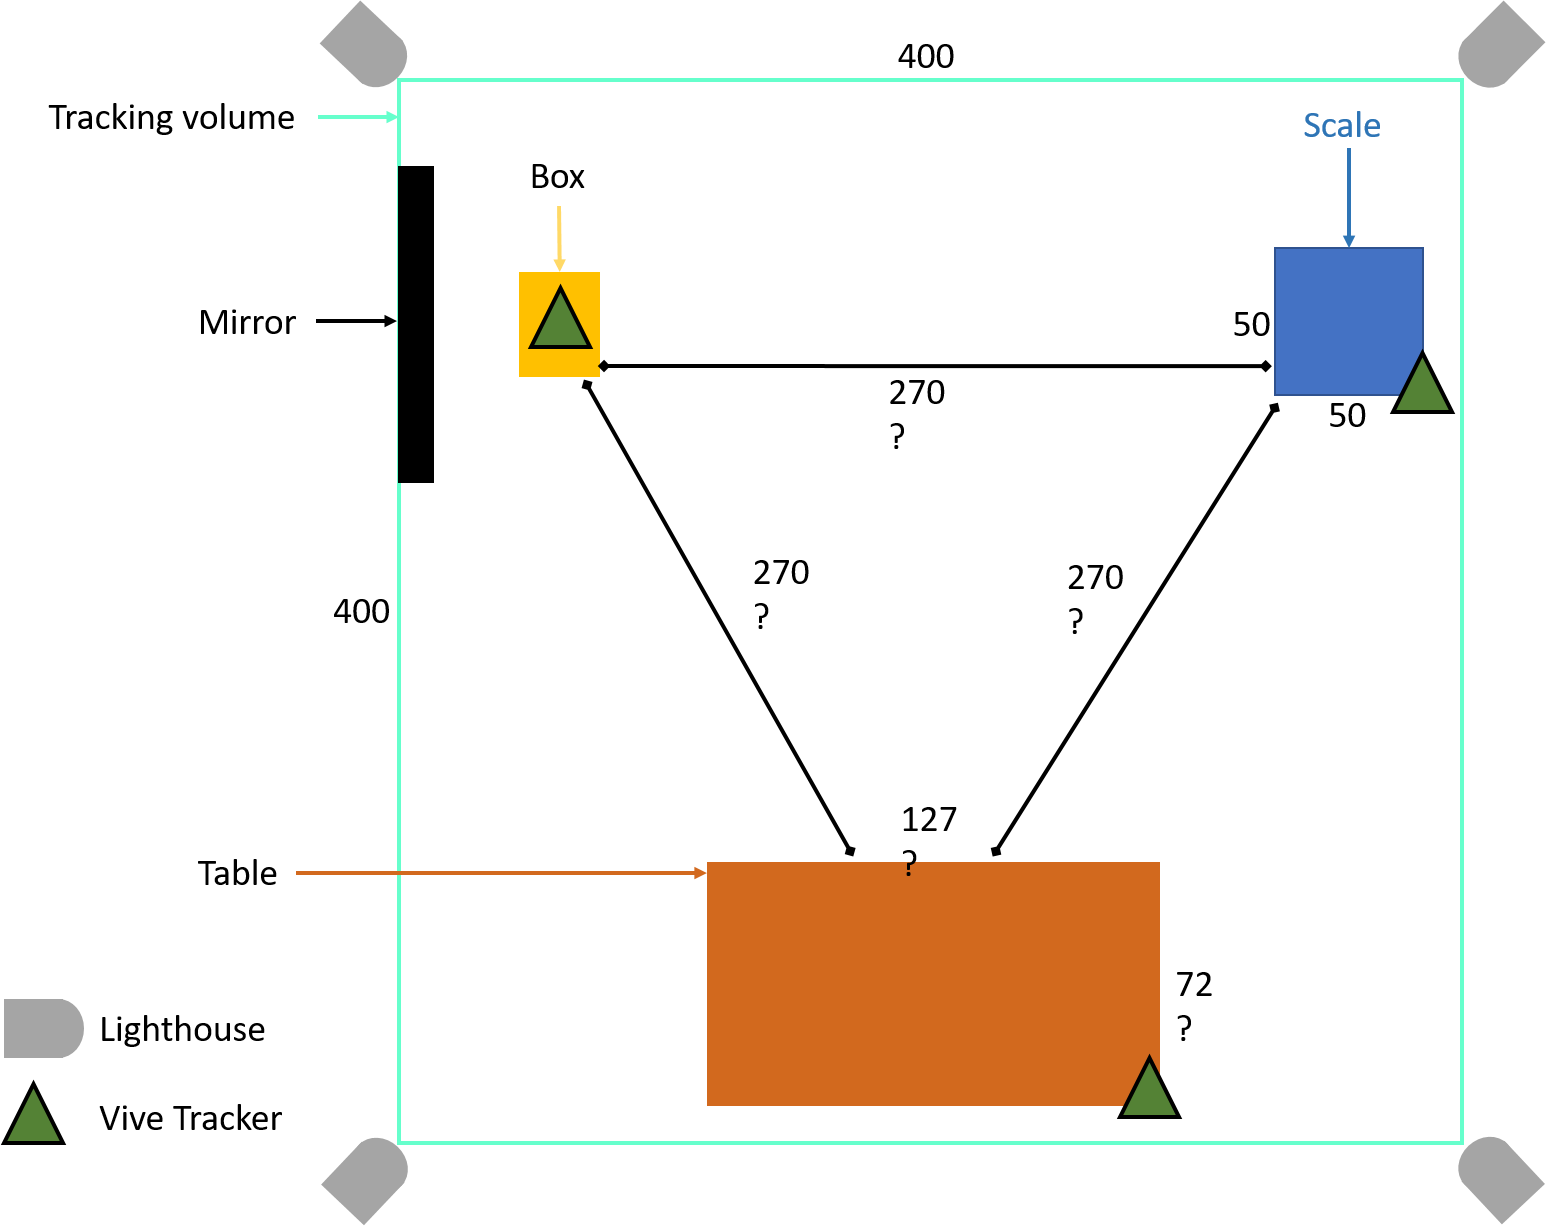
\includegraphics[width=\textwidth]{figures/study_setting.png}
	\caption[study setting]{study setting}
	\label{fig:study_setting}
\end{figure}

\begin{figure}[htb]
	\centering
	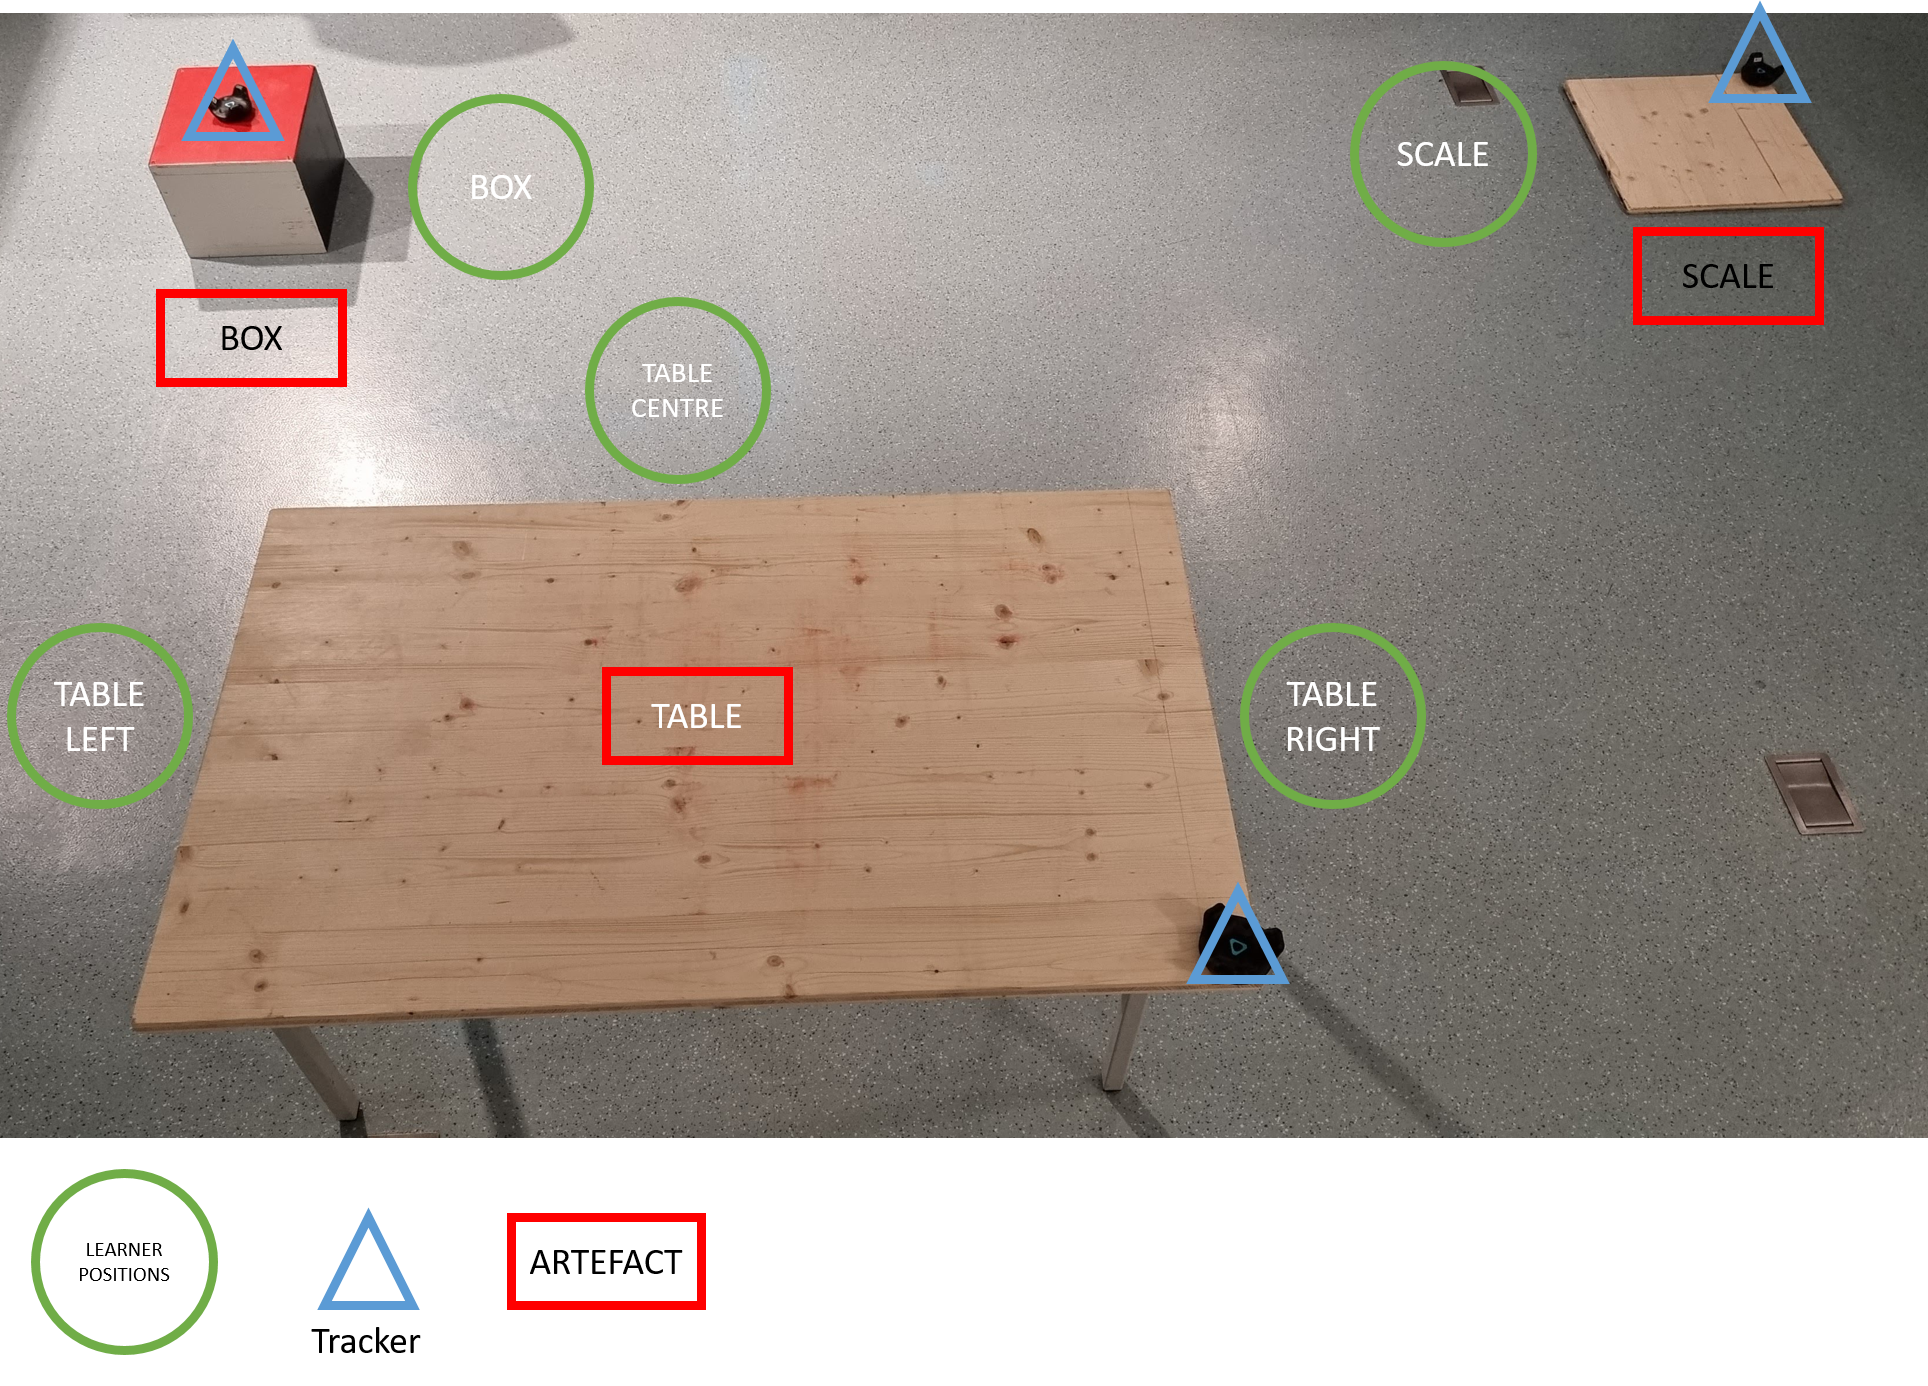
\includegraphics[width=\textwidth]{figures/learner_positions.png}
	\caption[Description of tasks]{tasks}
	\label{fig:learner_positions}
\end{figure}

\begin{figure}[htb]
	\centering
	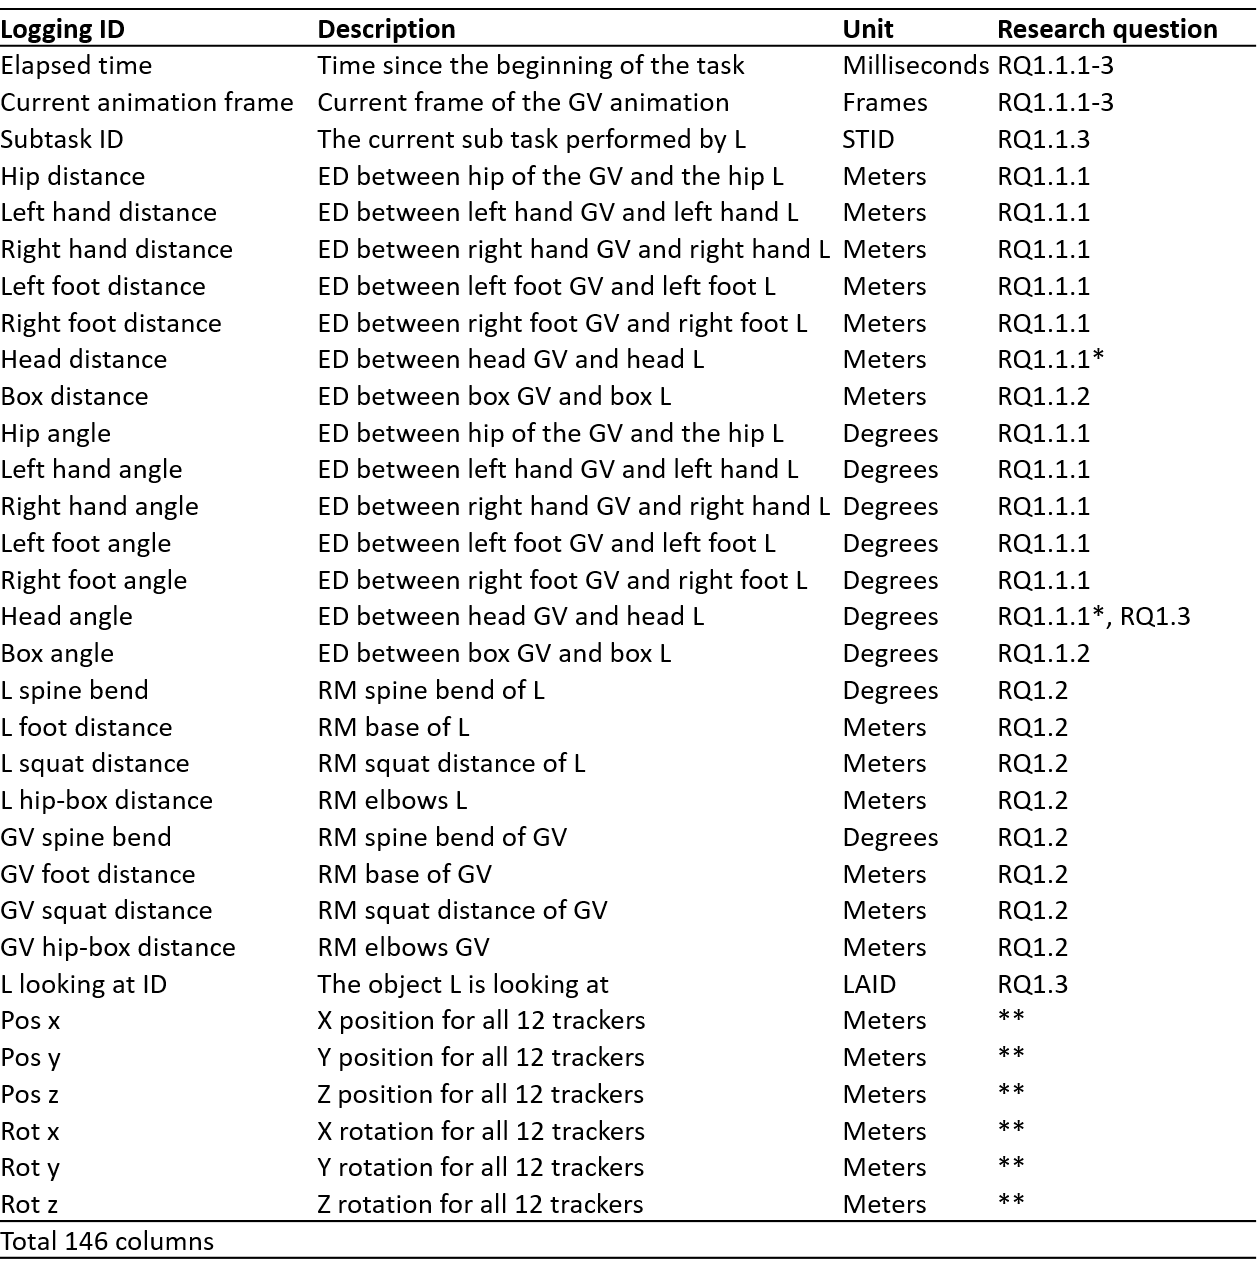
\includegraphics[width=\textwidth]{figures/logging_detail.png}
	\caption[logging detail]{Detailed overview of logs produced by \exgo\ per frame. L: learner, GV guidance visualistion, ED: euclidean distance. *head position and rotation is biased in exo-centric conditions because of multiple GV the L can focus on. **All trackers are logged for backup reasons: after the study is conducted a measurement can become interesting that was not of imporance before. With these values any measurement can be calculated post-study.}
	\label{fig:logging_detail}
\end{figure}

\begin{table}[htb]
	\centering
	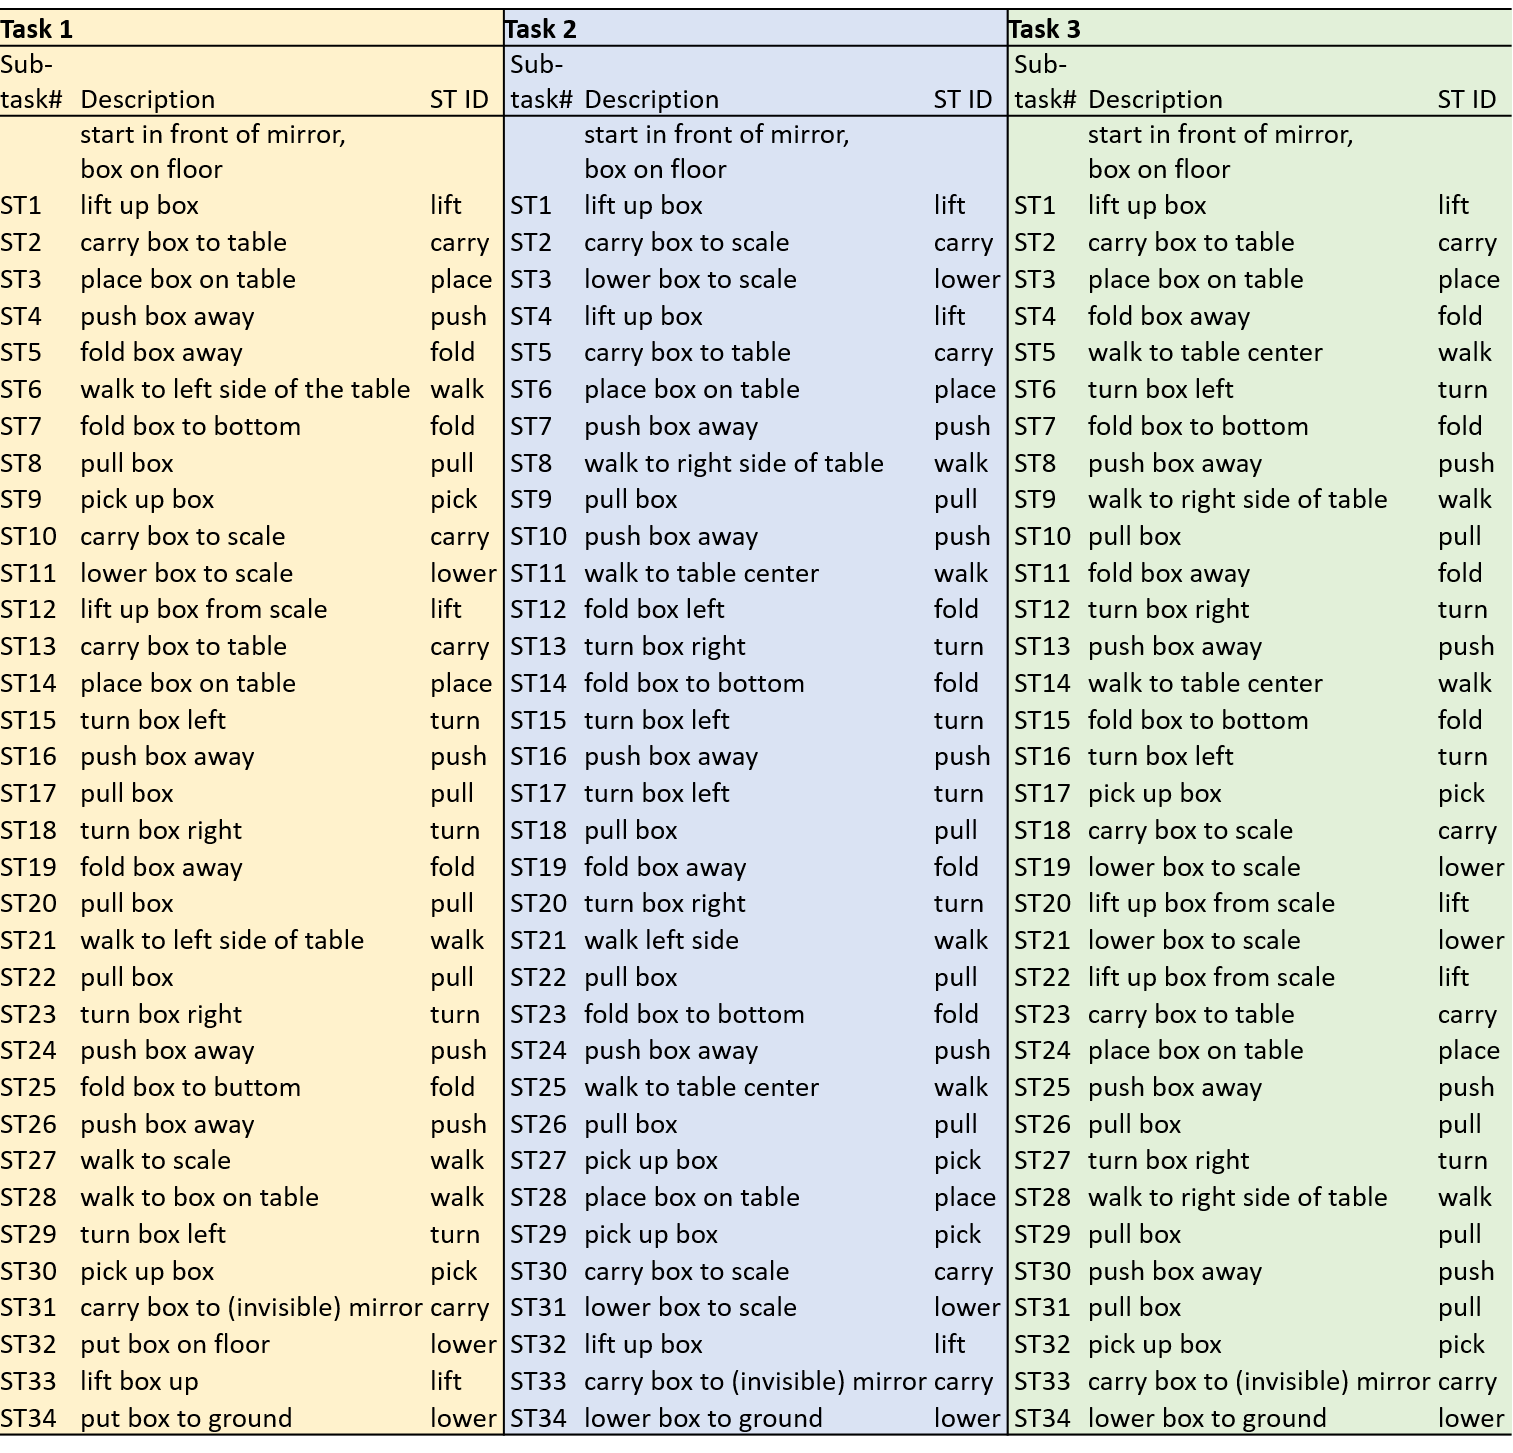
\includegraphics[width=\textwidth]{figures/tasks.png}
	\caption[Description of tasks]{tasks}
	\label{tab:tasks}
\end{table}

\begin{table}[htb]
	\centering
	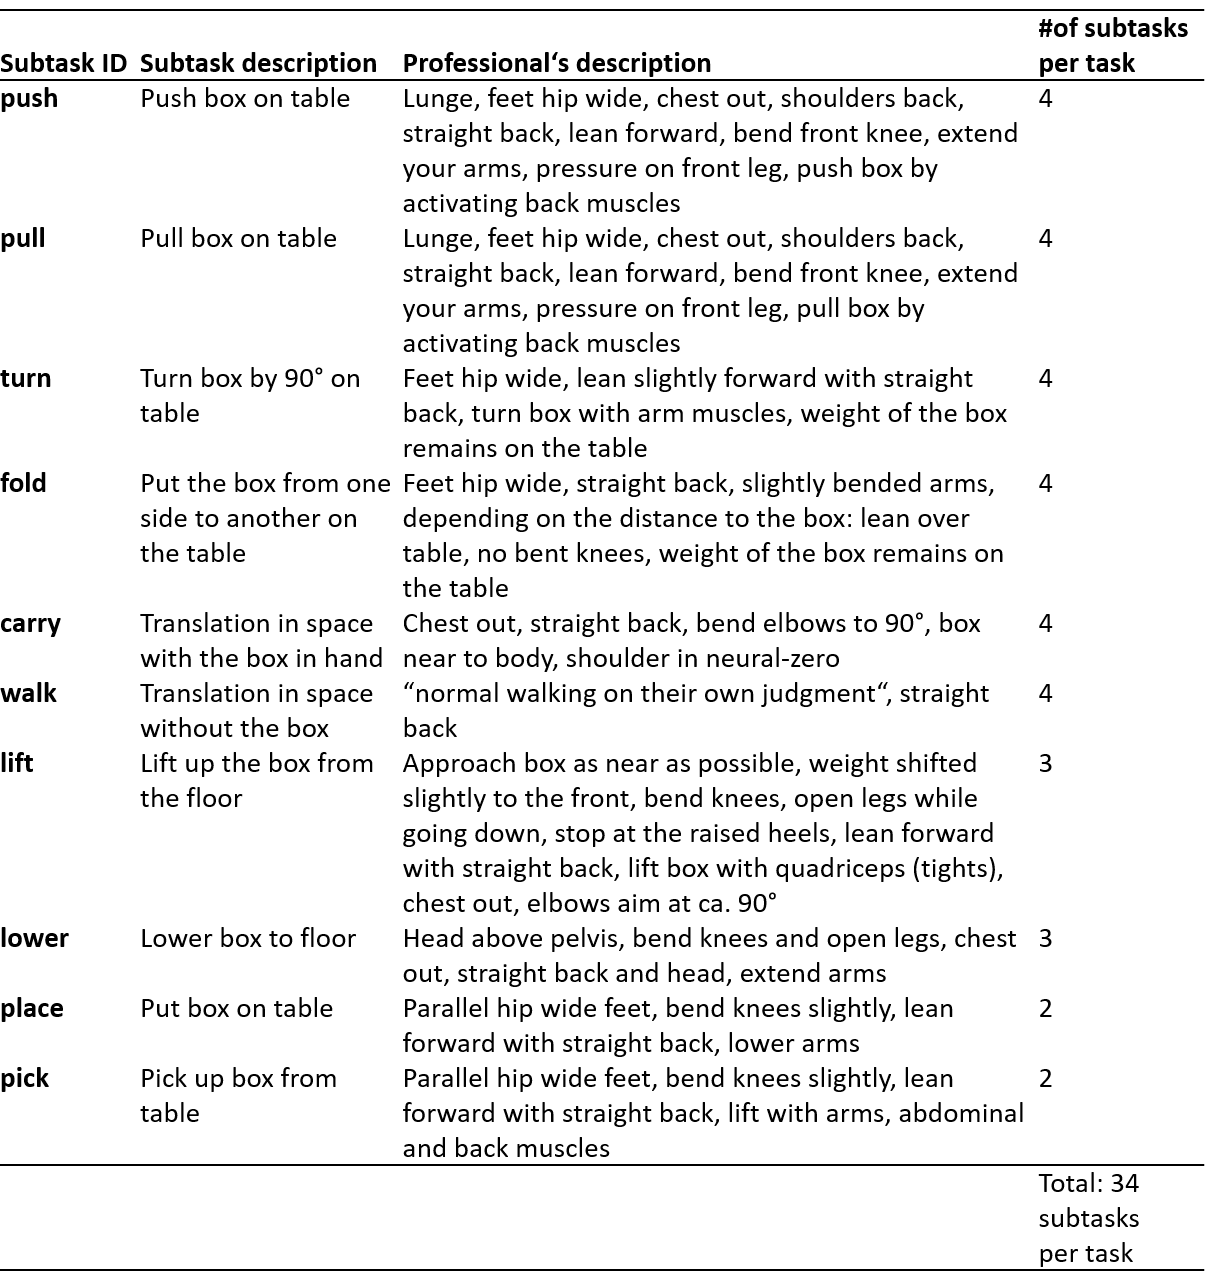
\includegraphics[width=\textwidth]{figures/sub_tasks_definition.png}
	\caption[Description of sub-tasks]{subtasks}
	\label{tab:sub-tasks}
\end{table}

\begin{figure}[htb]
	\centering
	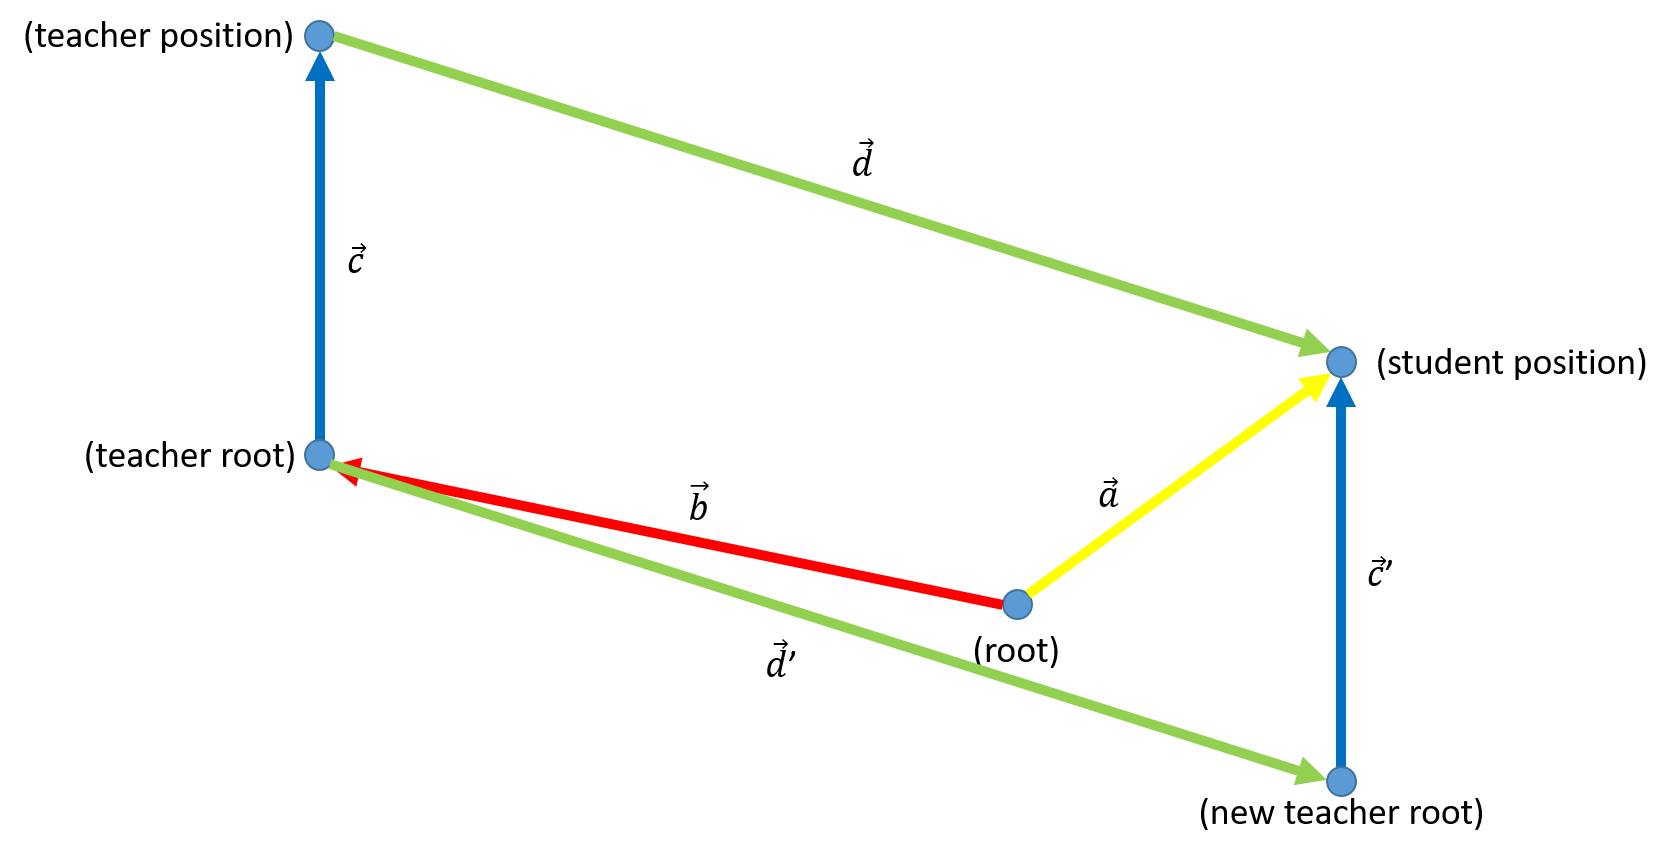
\includegraphics[width=\textwidth]{figures/shift_calc.png}
	\caption[shift calc]{shift calc}
	\label{fig:shift_calc}
\end{figure}



\begin{figure}[htb]
	\centering
	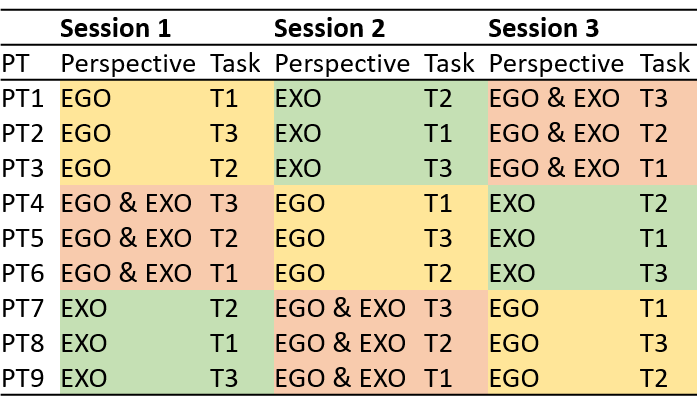
\includegraphics[width=0.5\textwidth]{figures/study_session_plan.png}
	\caption[session plan]{session plan}
	\label{fig:study_session_plan}
\end{figure}

tasks\\
procedure\\
geplante evaluierung\\
limitations\\
bezug zwischen messungen und forschungsfragen\\
triangulation nutzen wo sinnvoll\\
